\section{Table Understanding and Question Answering}
\label{sec:table}

Tables present unique challenges for document understanding: they encode structured relational data with implicit row-column dependencies, header hierarchies, and cell-level semantics that are easily lost when linearized into text. This section traces the evolution of table understanding through three stages (\cref{fig:table_stages}): structure-aware representation learning, generation enhancement and modular reasoning, and verifiable reasoning with multimodal understanding.

\subsection{Structure-Aware and Table Semantic Modeling}

Early research recognized that simple table linearization weakened the ability to model row-column relationships and cell dependencies. Work in this stage concentrated on structure-aware representation learning and benchmark construction.

Intermediate pre-training approaches significantly improved table understanding capabilities. Understanding Tables with Intermediate Pre-training \cite{eisenschlos2020understanding} and OmniTab \cite{jiang2022omnitab} introduced large-scale intermediate pre-training and multi-task pre-training to enhance understanding of table structures, numerical relationships, and linguistic alignment. Representations for QA from Documents with Tables and Text \cite{zayats2021representations} and SoarGraph \cite{zhu2023soargraph} emphasized joint modeling of tables and surrounding text, with SoarGraph capturing cross-modal semantic dependencies through graph-structured representations.

Reasoning capabilities were enhanced through specialized pre-training objectives. ReasTAP \cite{liu2023reastap} integrated table reasoning skills during pre-training via synthetic reasoning examples. FORTAP \cite{cheng2022fortap} leveraged spreadsheet formulas for numerical-reasoning-aware table pre-training. At the task level, AIT-QA \cite{katsis2022ait}, FeTaQA \cite{nan2022fetaqa}, and Arxiv Tables \cite{konopka2023arxiv} revealed limitations of traditional methods in complex industry tables, free-form table QA, and long-document table-text associations.

Visual document understanding expanded table research to document images. Visual Understanding of Complex Table Structures \cite{raja2022visual} and HTAN \cite{wu2025htan} proposed robust visual structure modeling for irregular and hierarchical tables. Analytical studies \cite{singha2023tabular,zhao2023large} revealed the sensitivity of LLMs to table representation formats and structural noise, pointing out constraints on their table parsing capabilities.

\subsection{Generation Enhancement and Modular Reasoning}

After establishing fundamental table structure modeling, research shifted toward leveraging LLM generative capabilities through modular, decomposed, and generation-enhanced strategies.

Table instruction tuning emerged as a key paradigm. Table-GPT \cite{peng2023table} performed ``table-tuning'' on general-purpose LLMs using large-scale synthetic table task data. TableGPT2 \cite{su2024tablegpt2} introduced specialized table encoders and multimodal pre-training for complex real-world tables. Rethinking Table Instruction Tuning \cite{deng2025rethinking} systematically analyzed hyperparameter and training scale impacts on performance and generalization.

Modular organization of the generation process enabled more sophisticated reasoning. Localize, Retrieve and Fuse (TAG-QA) \cite{zhao2023localize} supported free-form table QA through a three-stage framework. MFORT-QA \cite{guan2024mfort} combined few-shot learning with multi-hop Chain-of-Thought for cross-table reasoning. Large Language Models are Versatile Decomposers \cite{ye2023large} proposed using LLMs as question and evidence decomposers through a ``decompose-then-reason'' approach.

Input organization and noise suppression techniques improved practical applicability. TACR \cite{wu2024table} utilized table-question alignment for fine-grained cell selection. CABINET \cite{patnaik2024cabinet} reduced interference from irrelevant content through unsupervised relevance scoring. TabSQLify \cite{nahid2024tabsqlify} decomposed large tables into question-relevant sub-tables to reduce context length burdens.

Advanced reasoning methods integrated tables into the reasoning chain. Chain-of-table \cite{zhang2023chainoftable} proposed evolving tables in the reasoning chain. DePlot \cite{liu2023deplot} achieved visual language reasoning through plot-to-table translation. MultiHiertt \cite{wang2023multihiertt} provided numerical reasoning benchmarks for multi-hierarchical tables. Table as Thought \cite{huang2023tableasthought} organized the reasoning process in tabular form to enhance LLM reasoning.

\subsection{Verifiable Reasoning and Multimodal Table Understanding}

Recent research has focused on the verifiability of reasoning processes, execution consistency, and cross-modal reliability to build interpretable and trustworthy table QA systems.

Inference-time scaling and tool integration have improved reasoning capabilities. Table-R1 \cite{yang2025tablegpt1} proposed inference-time scaling for table reasoning through post-training strategies. Weaver \cite{weaver2025} combined SQL with LLMs to dynamically process structured and unstructured data. TableGPT-R1 \cite{yang2025tablegpt} introduced reinforcement learning to mitigate limitations of supervised fine-tuning in multi-step reasoning.

Interpretable reasoning frameworks provide explicit execution trajectories. Interpretable LLM-based Table QA \cite{nguyen2024interpretable} proposed Plan-of-SQLs (POS) to decompose queries into executable SQL sub-steps. Multi-LLM Agent QA over Tabular Data \cite{bangar-etal-2025-exploration} completed planning, code generation, and debugging through multi-agent collaboration.

Tool and execution enhancement approaches strengthen reliability. OpenTab \cite{kong2024opentab} combined table retrieval with SQL execution. TAT-LLM \cite{zhu2024tat} and MATATA \cite{vinayagame2025matata} strengthened discrete and mathematical reasoning through step-wise pipelines. TaPERA \cite{zhao2024tapera} improved trustworthiness through content planning and execution-driven reasoning.

Multimodal table understanding addresses visual table scenarios. TabIQA \cite{nguyen2023tabiqa}, ExpliCIT-QA \cite{hormazabal2025explicit}, and TabPedia \cite{zhao2024tabpedia} emphasized structural recovery, code-interpretable reasoning, and unified multi-task visual table understanding. Knowledge graph integration \cite{raj2024liberating,zhao2025tqagent} reduced hallucinations and supported multi-step tree-like reasoning.

\begin{figure*}[t]
\centering
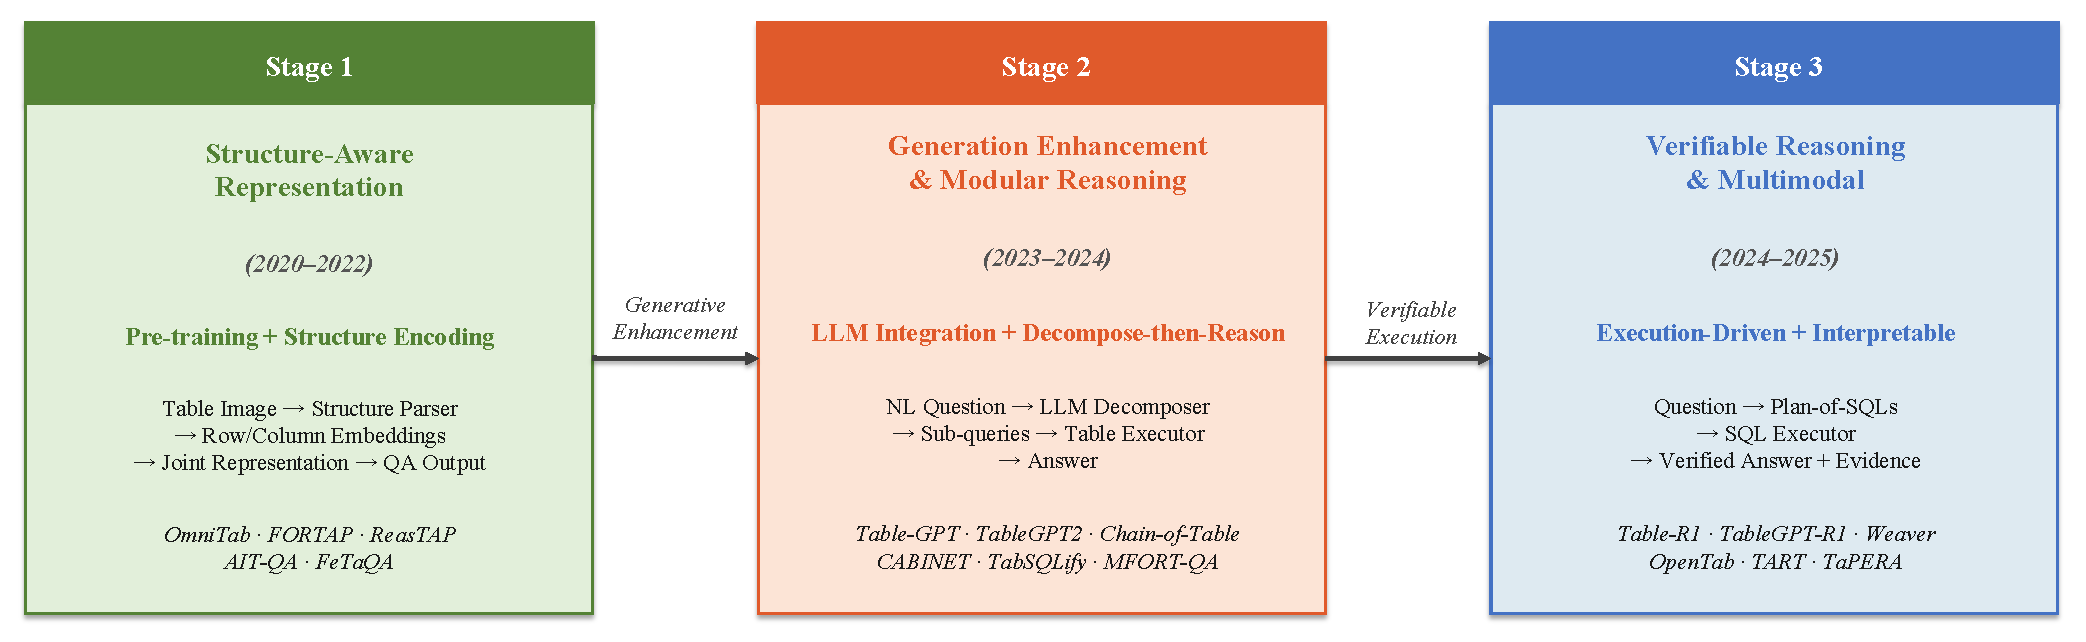
\includegraphics[
    width=0.95\textwidth,
    trim=0cm 0cm 0cm 0cm,
    clip
]{figs/fig05.pdf}
\caption{Three-stage evolution of table understanding and question answering (2020--2025): Stage~1 establishes structure-aware representation learning via pre-training and structure encoding; Stage~2 advances generation enhancement and modular reasoning through LLM integration and decompose-then-reason strategies; Stage~3 achieves verifiable reasoning and multimodal understanding driven by execution and interpretable inference.}
\label{fig:table_stages}
\end{figure*}
